% De single-cycle a pipeline (documento independiente).
% Compilar con ./build.sh (convierte el SVG a PDF y compila dos veces).
\documentclass[11pt,a4paper]{article}
\usepackage[utf8]{inputenc}
\usepackage[T1]{fontenc}
\usepackage[spanish,es-noquoting,es-tabla,es-nolists]{babel}
\usepackage{lmodern}
\usepackage{mathpazo}
\usepackage[scale=0.9]{tgheros}
\linespread{1.06}
\usepackage{microtype}
\usepackage[a4paper,margin=2.4cm]{geometry}
\usepackage{graphicx}
\usepackage{booktabs}
\usepackage{array}
\usepackage{caption}
\usepackage{enumitem}
\usepackage{xcolor}
\usepackage{listings}
\usepackage[most]{tcolorbox}
\usepackage{titlesec}
\usepackage[hidelinks]{hyperref}

\graphicspath{{figs/}}
\definecolor{hhblue}{RGB}{11,111,184}

\captionsetup{labelfont={bf,sf,color=hhblue},textfont={bf,sf,small},labelsep=quad,
  figurename=Figura,tablename=Tabla}

\titleformat{\section}{\sffamily\bfseries\Large}{\thesection}{0.7em}{\color{hhblue}}
\titleformat{\subsection}{\sffamily\bfseries\large}{\thesubsection}{0.7em}{\color{hhblue}}
\titlespacing*{\section}{0pt}{3.2ex plus 1ex minus .2ex}{1.6ex plus .2ex}
\titlespacing*{\subsection}{0pt}{2.6ex plus 1ex minus .2ex}{1.2ex plus .2ex}

% nombres de señales en cursiva; módulos y archivos en monoespaciado
\newcommand{\sig}[1]{\textit{#1}}
\newcommand{\ins}[1]{\texttt{#1}}

\lstdefinestyle{vlog}{language=Verilog, basicstyle=\ttfamily\footnotesize, columns=fullflexible,
  keywordstyle=\color{hhblue}\bfseries, commentstyle=\color{black!55}\itshape,
  showstringspaces=false, keepspaces=true, upquote=true, breaklines=true}
\newtcblisting{hdl}{listing only, breakable, colback=black!3, colframe=black!35,
  boxrule=0.4pt, arc=1.5pt, left=4pt, right=4pt, top=2pt, bottom=2pt,
  listing options={style=vlog}}

\setlist{itemsep=1pt, topsep=3pt}
\setlist[itemize]{label=\textbullet}
\renewcommand{\arraystretch}{1.15}

\title{\sffamily\bfseries\color{hhblue} De single-cycle a pipeline (RISC-V)}
\author{}
\date{}

\begin{document}
\maketitle

Guía de los cambios hechos para convertir el procesador RISC-V single-cycle en uno segmentado de 5 etapas (IF, ID, EX, MEM, WB) con manejo de hazards. Cada paso agrupa uno o varios commits; las correcciones menores no se detallan.

\textbf{Convención de nombres:} el sufijo de cada señal indica la etapa en la que vive (\textbf{F}etch, \textbf{D}ecode, \textbf{E}xecute, \textbf{M}emory, \textbf{W}riteback). Ej.: \sig{RegWriteW} es el \sig{RegWrite} que llega a la etapa WB.

\begin{center}
\begin{tabular}{@{}cll@{}}
\toprule
Paso & Qué se agrega & Commits \\
\midrule
0 & Base single-cycle & \ins{be12a76} \\
1 & Registros de pipeline en el datapath & \ins{fca53aa} \\
2 & Registros de pipeline en el controller & \ins{9ca1706} \\
3 & Conexión en \ins{riscv.v} & \ins{bdf4e5e} \\
4 & Flops con \sig{enable} y \sig{clear} & \ins{ab14e98} \\
5 & Hazard unit & \ins{223f612}, \ins{be83e01} \\
6 & Hazard unit integrada en datapath, controller y top & \ins{0a26a3b}, \ins{90981cc}, \ins{869f719} \\
\bottomrule
\end{tabular}
\end{center}

%-----------------------------------------------------------------
\section{Paso 0 --- Base single-cycle}

Punto de partida: un procesador de ciclo único con \ins{riscvsingle}, \ins{controller}, \ins{datapath}, \ins{maindec}, \ins{aludec}, \ins{alu}, \ins{regfile}, \ins{extend}, \ins{imem}, \ins{dmem}, etc. Soporta \ins{lw}, \ins{sw}, \ins{beq}, tipo R, tipo I y \ins{jal}.

En un solo ciclo ocurre todo: se lee la instrucción, se decodifica, se ejecuta, se accede a memoria y se escribe el resultado. El período de reloj lo limita la ruta más larga (la de \ins{lw}).

\begin{figure}[h]
\centering
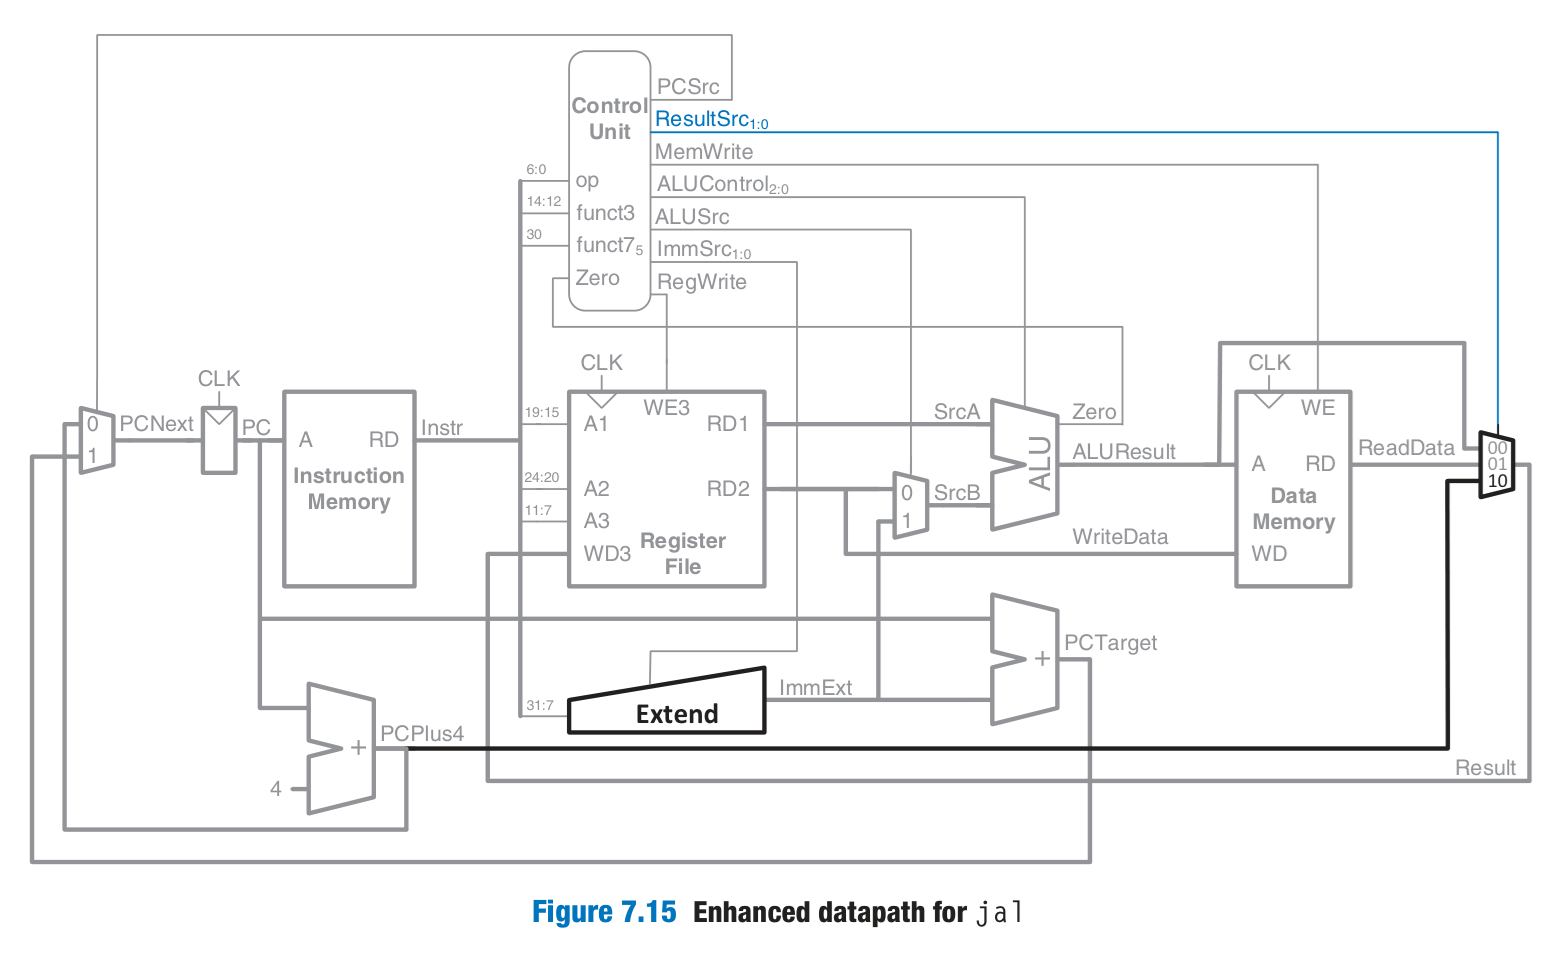
\includegraphics[width=\linewidth,trim=0 68.3bp 0 0,clip]{singlecycle-processor}
\caption{Procesador single-cycle.}
\end{figure}

\begin{figure}[h]
\centering
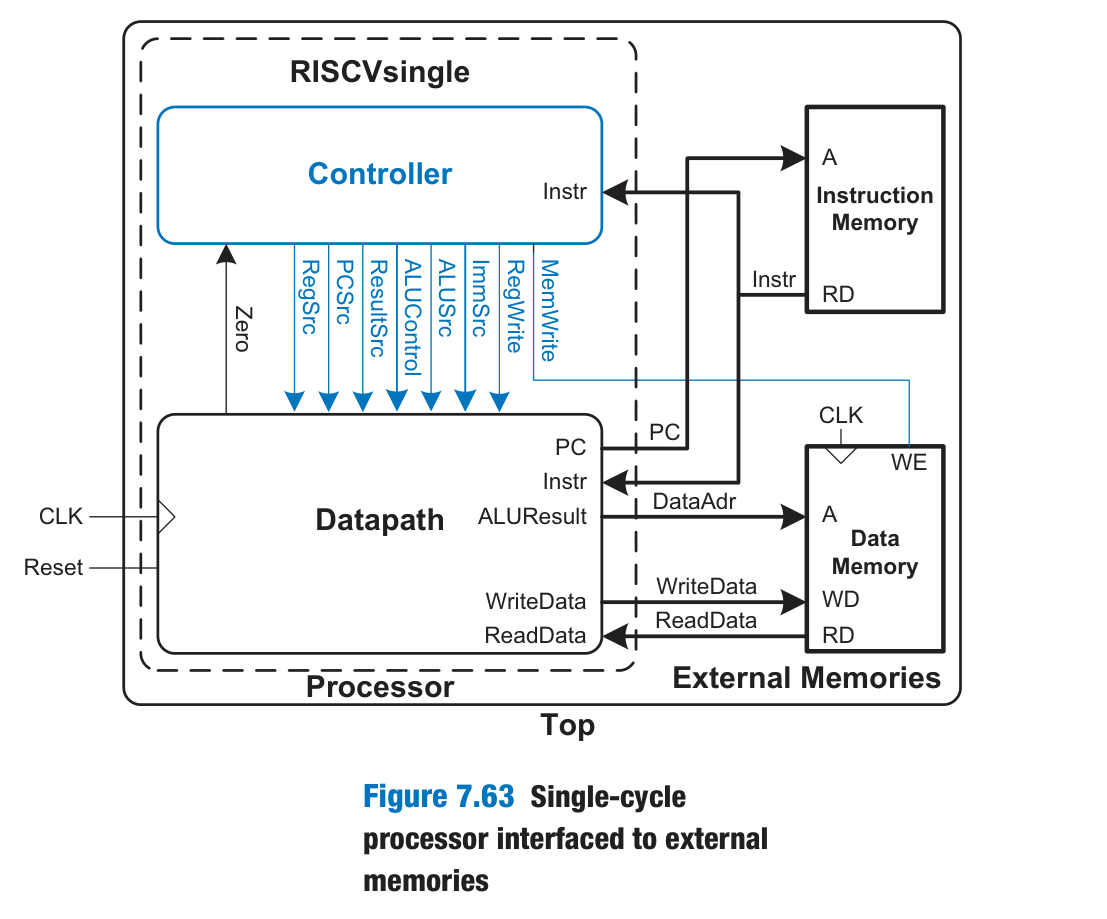
\includegraphics[width=0.8\linewidth,trim=0 133.5bp 0 0,clip]{singlecycle-top}
\caption{Top single-cycle.}
\end{figure}

%-----------------------------------------------------------------
\section{Paso 1 --- Registros de pipeline en el datapath}

Se divide el datapath en 5 etapas separadas por 4 registros de pipeline (se usa \ins{flopr} con el bus concatenado):

\begin{center}
\begin{tabular}{@{}ll@{}}
\toprule
Registro & Contiene \\
\midrule
IF/ID (\ins{regD}) & \sig{InstrF}, \sig{PCF}, \sig{PCPlus4F} \\
ID/EX (\ins{regE}) & \sig{RD1D}, \sig{RD2D}, \sig{PCD}, \sig{RdD}, \sig{ImmExtD}, \sig{PCPlus4D} \\
EX/MEM (\ins{regM}) & \sig{ALUResultE}, \sig{WriteDataE}, \sig{RdE}, \sig{PCPlus4E} \\
MEM/WB (\ins{regW}) & \sig{ALUResultM}, \sig{ReadDataM}, \sig{RdM}, \sig{PCPlus4M} \\
\bottomrule
\end{tabular}
\end{center}

Cambios importantes respecto al single-cycle:
\begin{itemize}
  \item \textbf{Renombrado por etapa} de todas las señales (\sig{ALUResult} $\to$ \sig{ALUResultM}, \sig{Zero} $\to$ \sig{ZeroE}, etc.).
  \item \textbf{El sumador del branch target} (\ins{pcaddbranch}) pasó de Fetch a Execute: ahora usa \sig{PCE} + \sig{ImmExtE} y produce \sig{PCTargetE}. El \sig{PCSrc} que elige el siguiente PC se resuelve en EX (\sig{PCSrcE}).
  \item \textbf{\sig{Rd} viaja con la instrucción} hasta WB, para que la escritura en el register file use el \sig{RdW} correcto y no el \sig{Rd} de la instrucción que está en Decode.
  \item \textbf{El register file escribe en el flanco de bajada} (\ins{negedge clk}), de modo que una instrucción en WB y otra en ID que lean el mismo registro en el mismo ciclo ven el valor nuevo (resuelve ese hazard sin lógica extra).
\end{itemize}

\begin{figure}[h]
\centering
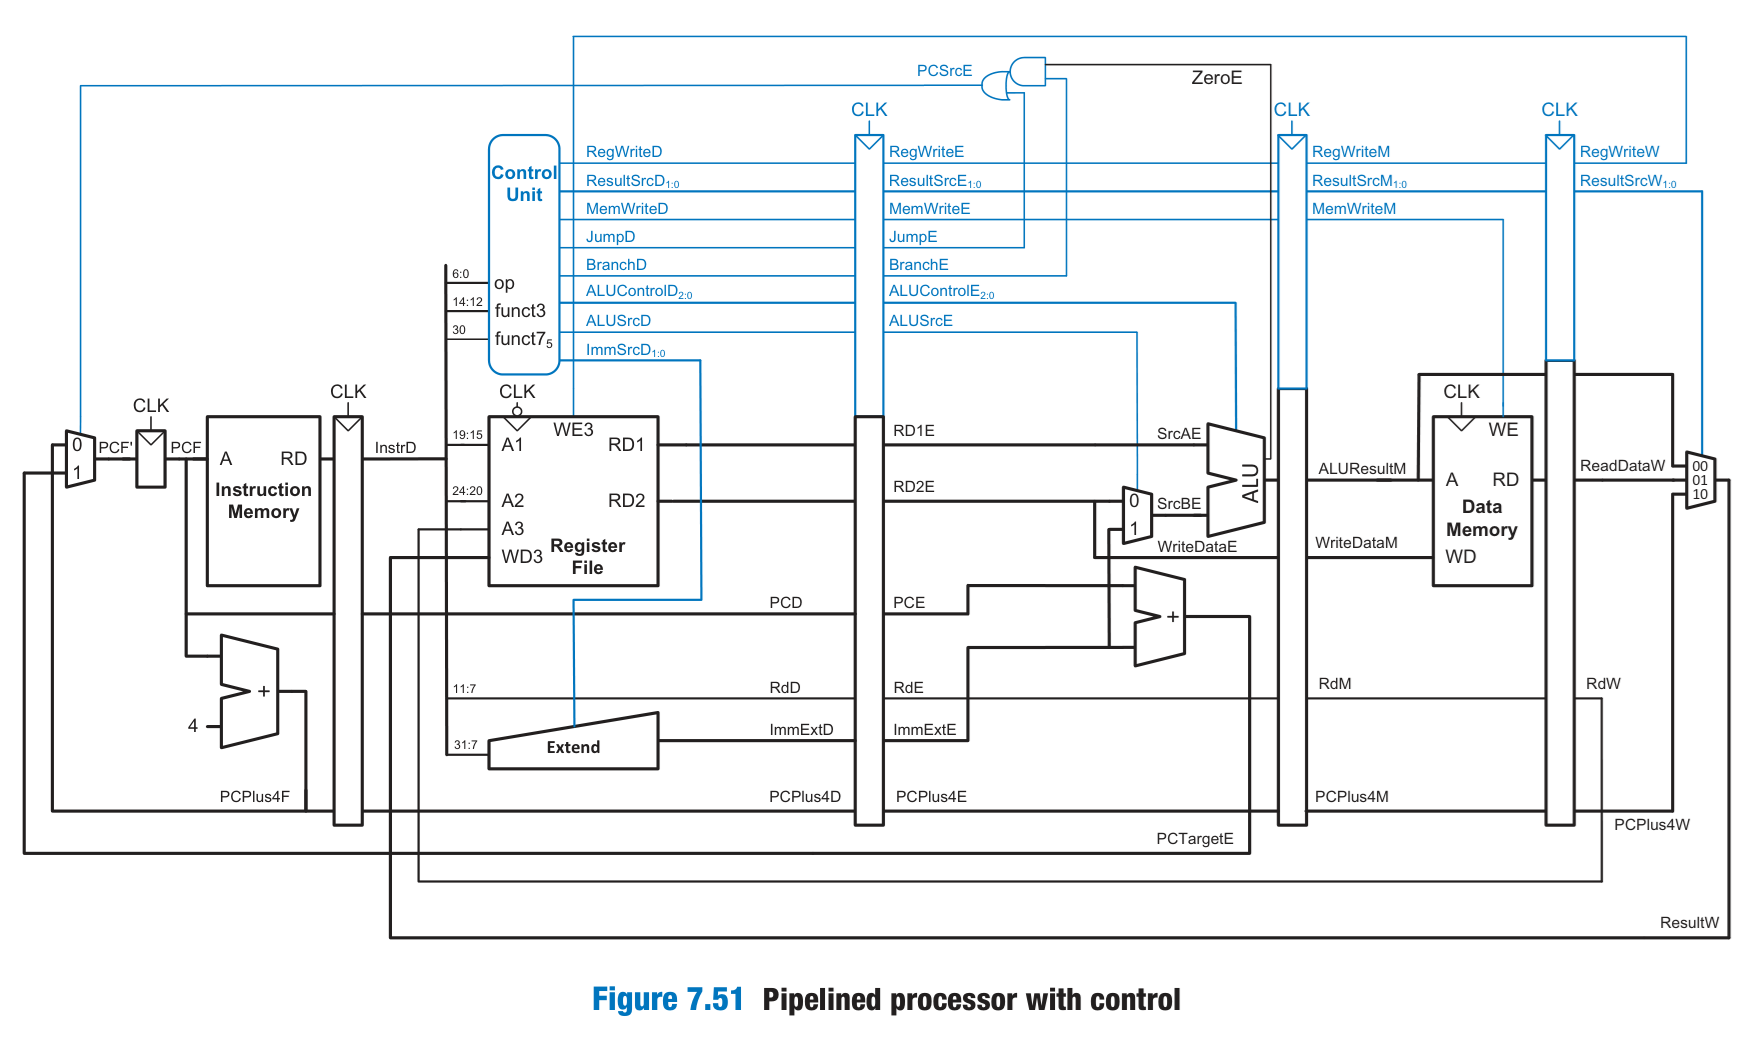
\includegraphics[width=\linewidth,trim=0 80.3bp 0 0,clip]{pipeline-processor-no-hazards}
\caption{Procesador pipeline sin hazards.}
\end{figure}

%-----------------------------------------------------------------
\section{Paso 2 --- Registros de pipeline en el controller}

Las señales de control se generan en Decode y deben acompañar a la instrucción por el pipeline. El controller ahora recibe \sig{clk}/\sig{reset} y tiene sus propios registros:

\begin{center}
\begin{tabular}{@{}ll@{}}
\toprule
Registro & Señales \\
\midrule
ID/EX & \sig{RegWrite}, \sig{ResultSrc}, \sig{MemWrite}, \sig{Jump}, \sig{Branch}, \sig{ALUControl}, \sig{ALUSrc} \\
EX/MEM & \sig{RegWrite}, \sig{ResultSrc}, \sig{MemWrite} \\
MEM/WB & \sig{RegWrite}, \sig{ResultSrc} \\
\bottomrule
\end{tabular}
\end{center}

Cada señal se consume en la etapa donde hace falta y ya no se propaga más:
\begin{itemize}
  \item \sig{ImmSrcD}: Decode.
  \item \sig{ALUSrcE}, \sig{ALUControlE}: Execute.
  \item \sig{PCSrcE} = \sig{BranchE} $\wedge$ \sig{ZeroE} $\vee$ \sig{JumpE}: Execute (antes se calculaba en el mismo ciclo que todo lo demás).
  \item \sig{MemWriteM}: Memory.
  \item \sig{RegWriteW}, \sig{ResultSrcW}: Writeback.
\end{itemize}

%-----------------------------------------------------------------
\section{Paso 3 --- Conexión en \texttt{riscv.v}}

\begin{itemize}
  \item \ins{riscvsingle.v} se reemplaza por \ins{riscv.v}, que conecta controller y datapath con los nuevos nombres.
  \item El datapath expone \sig{InstrD} como salida: el controller decodifica \sig{op}, \sig{funct3} y \sig{funct7b5} desde la instrucción \textbf{en Decode} (no la de Fetch).
  \item \ins{top.v} se ajusta a los nuevos puertos (\sig{PCF}, \sig{InstrF}, \sig{ALUResultM}, \sig{WriteDataM}, \sig{MemWriteM}, \sig{ReadDataM}).
\end{itemize}

Hasta aquí el pipeline funciona \textbf{solo para programas sin dependencias} entre instrucciones consecutivas (sin hazards de datos ni de control).

%-----------------------------------------------------------------
\section{Paso 4 --- Flops con \sig{enable} y \sig{clear}}

Para poder congelar y vaciar etapas se agregan tres variantes de \ins{flopr}:

\begin{center}
\begin{tabular}{@{}lll@{}}
\toprule
Módulo & Comportamiento & Uso \\
\midrule
\ins{flopenr} & Solo captura \sig{d} si \sig{en} & PC (\sig{StallF}) \\
\ins{floprc} & Pone \sig{q} = 0 si \sig{clear} & ID/EX (\sig{FlushE}) \\
\ins{flopenrc} & \sig{en} y \sig{clear} combinados & IF/ID (\sig{StallD} y \sig{FlushD}) \\
\bottomrule
\end{tabular}
\end{center}

%-----------------------------------------------------------------
\section{Paso 5 --- Hazard unit}

Módulo nuevo \ins{hazard.v}, puramente combinacional. Resuelve tres casos.

\subsection{Hazards de datos por forwarding (RAW)}

Si una instrucción en EX necesita un registro que una instrucción posterior (en MEM o WB) todavía no escribió, se le adelanta el valor. \sig{ForwardAE}/\sig{ForwardBE}:

\begin{center}
\begin{tabular}{@{}cl@{}}
\toprule
Valor & Fuente \\
\midrule
\ins{00} & Register file (\sig{RD1E}/\sig{RD2E}) \\
\ins{01} & \sig{ResultW} (de WB) \\
\ins{10} & \sig{ALUResultM} (de MEM) \\
\bottomrule
\end{tabular}
\end{center}

Condición: \sig{Rs1E} = \sig{RdM} $\wedge$ \sig{RegWriteM} (tiene prioridad MEM sobre WB) y \sig{Rs} $\neq$ \ins{x0}.

\subsection{Hazard de \texttt{lw} (stall)}

El dato de un \ins{lw} recién está disponible al final de MEM, así que ni el forwarding lo salva si la instrucción siguiente lo usa. Se detecta con:

\begin{hdl}
lwStallD = ResultSrcEb0 & ((Rs1D == RdE) | (Rs2D == RdE));
\end{hdl}

Acción: \sig{StallF} y \sig{StallD} congelan PC e IF/ID, y \sig{FlushE} inserta una burbuja en EX. Un ciclo después, el forwarding desde WB entrega el dato.

\subsection{Hazard de control (flush)}

El branch/jump se resuelve en EX, así que las 2 instrucciones siguientes ya se buscaron por error. Si \sig{PCSrcE} = 1, \sig{FlushD} y \sig{FlushE} las descartan.

\begin{center}
\begin{tabular}{@{}ll@{}}
\toprule
Salida & Condición \\
\midrule
\sig{StallF}, \sig{StallD} & \sig{lwStallD} \\
\sig{FlushD} & \sig{PCSrcE} \\
\sig{FlushE} & \sig{lwStallD} $\vee$ \sig{PCSrcE} \\
\bottomrule
\end{tabular}
\end{center}

%-----------------------------------------------------------------
\section{Paso 6 --- Integración de la hazard unit}

Se conecta todo lo anterior:
\begin{itemize}
  \item \textbf{Datapath}: nuevos puertos \sig{StallF}, \sig{StallD}, \sig{FlushD}, \sig{FlushE}, \sig{ForwardAE}, \sig{ForwardBE}. El PC pasa a \ins{flopenr}, IF/ID a \ins{flopenrc}, ID/EX a \ins{floprc}. Se agregan dos \ins{mux3} antes de la ALU (\ins{faemux} para \sig{SrcAE} y \ins{fbemux} para \sig{WriteDataE}, que luego pasa por el mux de \sig{ALUSrcE}) que eligen entre el register file, \sig{ResultW} y \sig{ALUResultM}. Se exponen \sig{Rs1D}, \sig{Rs2D}, \sig{Rs1E}, \sig{Rs2E}, \sig{RdE}, \sig{RdM}, \sig{RdW} hacia la hazard unit.
  \item \textbf{Controller}: el registro ID/EX pasa a \ins{floprc} con \sig{clear} = \sig{FlushE}, y expone \sig{RegWriteM} y \sig{ResultSrcEb0} hacia la hazard unit (\sig{RegWriteW} ya salía hacia el datapath).
  \item \textbf{\ins{riscv.v}}: instancia \ins{hazard} y cablea sus entradas/salidas entre controller y datapath.
\end{itemize}

\textit{Nota:} al hacer flush los registros se ponen en 0, es decir, una instrucción \ins{0x00000000}. Por eso \ins{maindec} recibió un caso \ins{7'b0000000} con controles en cero, para que esa ``instrucción nula'' no escriba registros ni memoria (y no genere \ins{x} en simulación).

\begin{figure}[h]
\centering
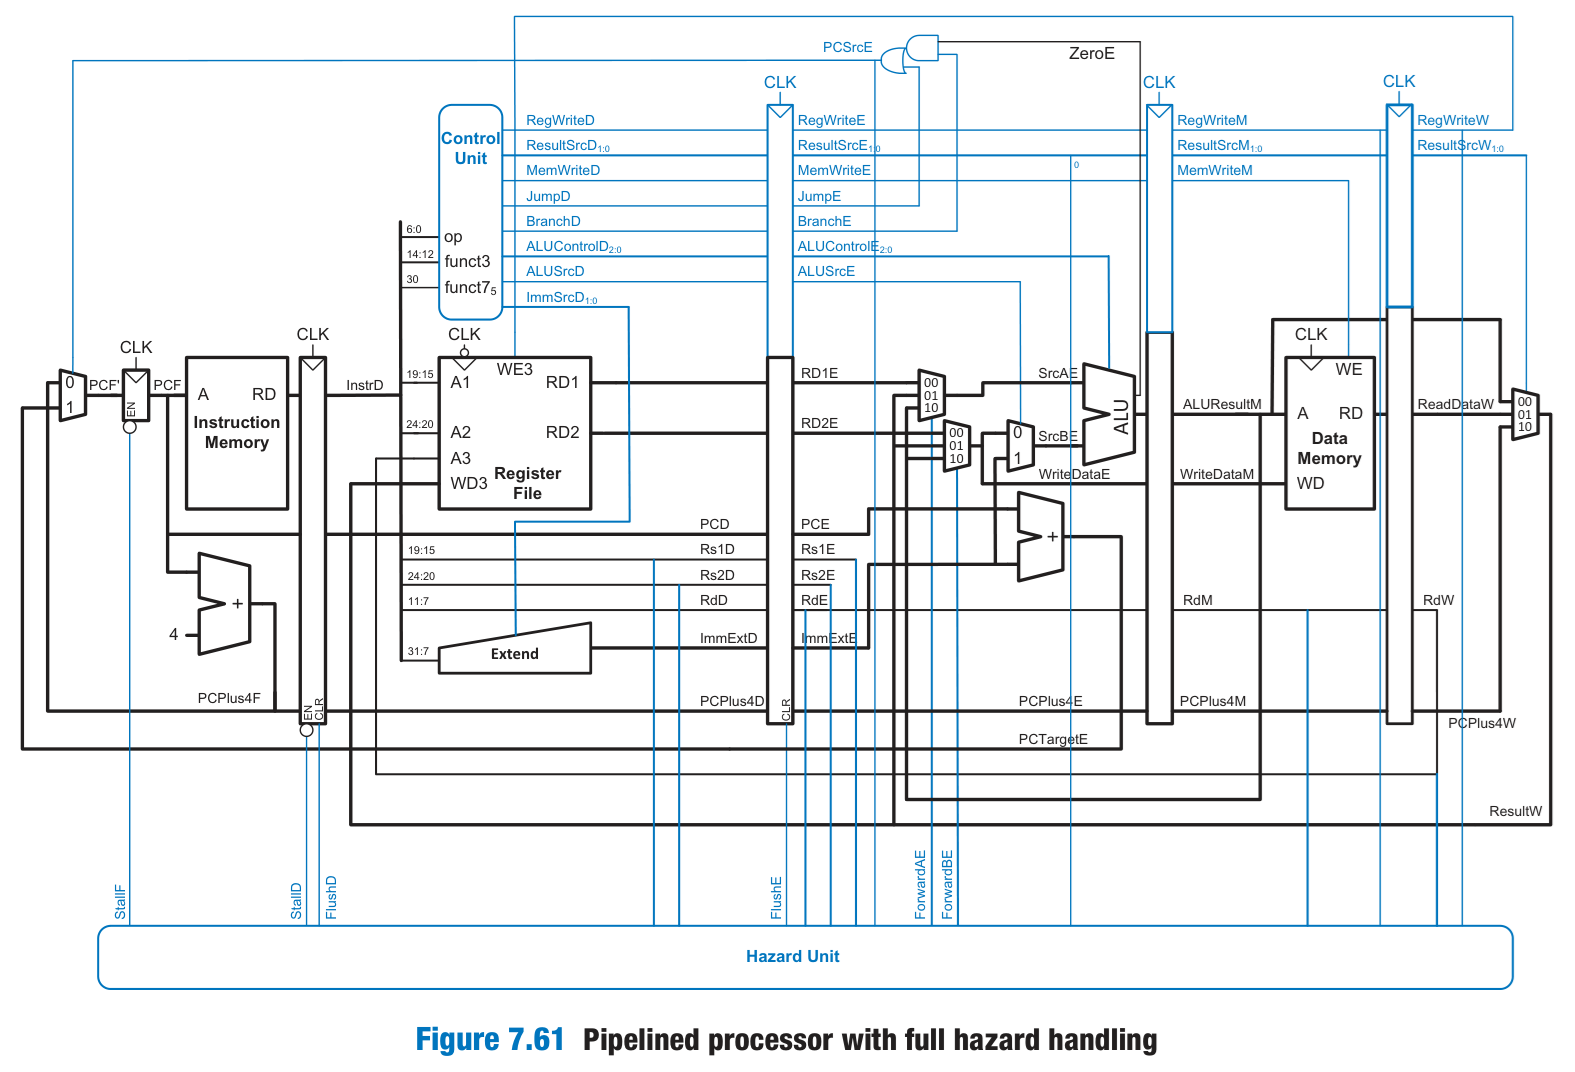
\includegraphics[width=\linewidth,trim=0 61.5bp 0 0,clip]{pipeline-processor-with-hazards}
\caption{Procesador pipeline con hazards.}
\end{figure}

\begin{figure}[h]
\centering
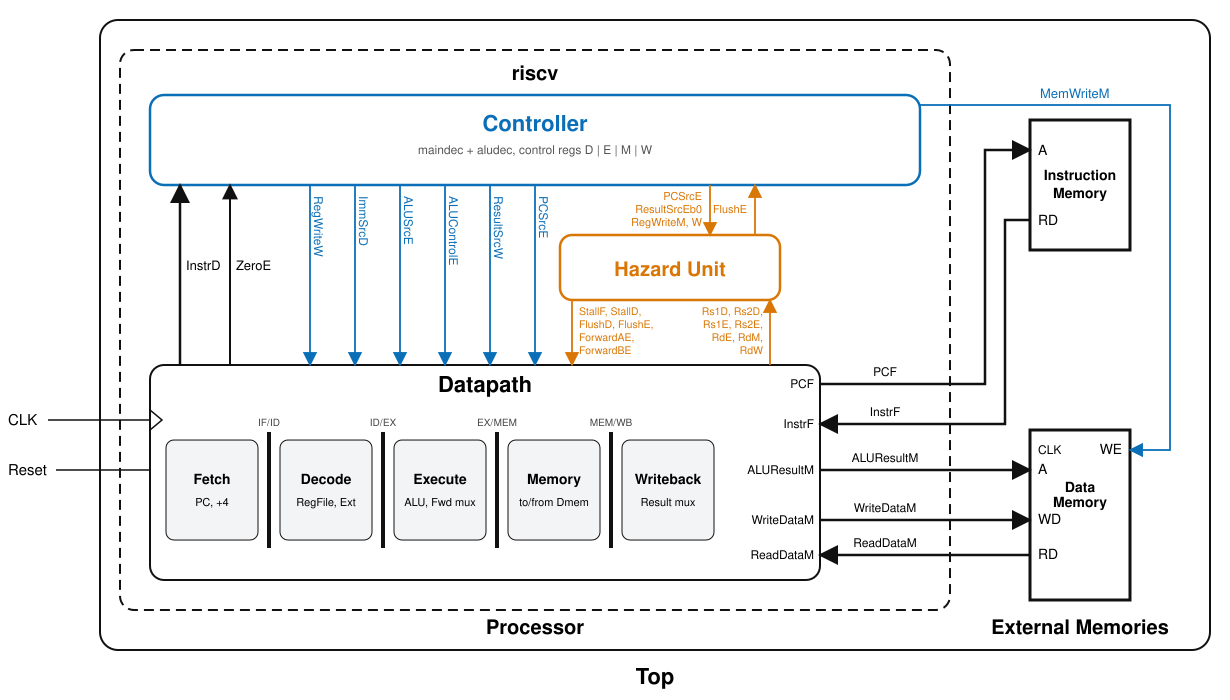
\includegraphics[width=\linewidth]{pipeline-top}
\caption{Top pipeline propio.}
\end{figure}

\end{document}
